\documentclass{article}
\usepackage[paperwidth=7.6cm,paperheight=12.8cm,margin=0pt]{geometry}
\usepackage{fontspec,tikz}
\usepackage[table]{xcolor}
\IfFontExistsTF{Helvetica Neue}
  {\setmainfont{Helvetica Neue}\setsansfont{Helvetica Neue}}
  {\IfFontExistsTF{Arial}{\setmainfont{Arial}\setsansfont{Arial}}{}}
\definecolor{navy}{HTML}{315E75}
\definecolor{teal}{HTML}{2E766E}
\definecolor{amber}{HTML}{A17431}
\definecolor{ink}{HTML}{2B3A42}
\definecolor{mute}{HTML}{7A8C94}
\definecolor{lightblue}{HTML}{EAF3F7}
\definecolor{lightteal}{HTML}{EDF6F2}
\definecolor{lightamber}{HTML}{FAF3E5}
\definecolor{lightrow}{HTML}{F7FAFB}
\definecolor{hairline}{HTML}{BDD0D8}
\pagestyle{empty}
\begin{document}
\noindent\hspace*{7mm}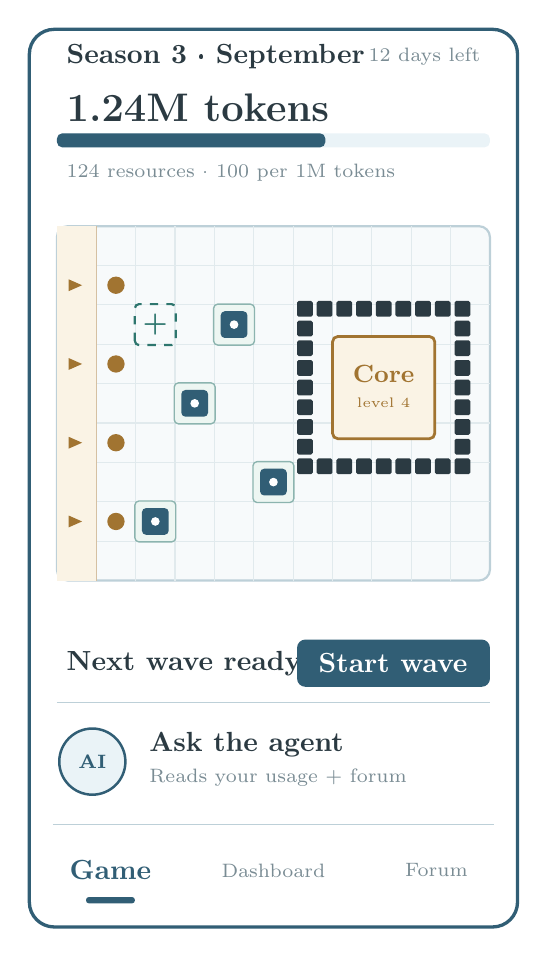
\begin{tikzpicture}[every node/.style={text=ink}]
\draw[draw=navy,line width=1.2pt,rounded corners=9pt] (0,0) rectangle (6.2,11.4);
% top block
\node[anchor=west,font=\bfseries] at (.35,11.05) {Season 3 · September};
\node[anchor=east,font=\scriptsize,text=mute] at (5.85,11.05) {12 days left};
\node[anchor=west,font=\Large\bfseries] at (.35,10.40) {1.24M tokens};
\fill[lightblue,rounded corners=2pt] (.35,9.90) rectangle (5.85,10.08);
\fill[navy,rounded corners=2pt] (.35,9.90) rectangle (3.76,10.08);
\node[anchor=west,font=\scriptsize,text=mute] at (.35,9.58) {124 resources · 100 per 1M tokens};
% ---- battlefield: a build plot you fill yourself, attacked from one side
\fill[lightrow,rounded corners=4pt] (.35,4.40) rectangle (5.85,8.90);
\draw[draw=hairline,line width=.8pt,rounded corners=4pt] (.35,4.40) rectangle (5.85,8.90);
% build grid: every cell can take a defence
\foreach \i in {1,...,10}{\draw[draw=hairline!45,line width=.4pt] ({.35+.5*\i},4.40) -- ({.35+.5*\i},8.90);}
\foreach \j in {1,...,8}{\draw[draw=hairline!45,line width=.4pt] (.35,{4.40+.5*\j}) -- (5.85,{4.40+.5*\j});}
% the single approach: everything arrives along the left edge
\fill[lightamber] (.35,4.40) rectangle (.85,8.90);
\draw[draw=amber!45,line width=.5pt] (.85,4.40) -- (.85,8.90);
\foreach \y in {5.15,6.15,7.15,8.15}{%
  \fill[amber] (.67,\y) -- (.50,\y+.075) -- (.50,\y-.075) -- cycle;
  \fill[amber] (1.10,\y) circle (.11);
}
% wall segments close off the compound, so a wave has to break through
\foreach \i in {0,...,8}{%
  \fill[ink,rounded corners=.6pt] ({3.40+.25*\i},5.75) rectangle ({3.60+.25*\i},5.95);
  \fill[ink,rounded corners=.6pt] ({3.40+.25*\i},7.75) rectangle ({3.60+.25*\i},7.95);
}
\foreach \j in {1,...,7}{%
  \fill[ink,rounded corners=.6pt] (3.40,{5.85+.25*\j-.10}) rectangle (3.60,{5.85+.25*\j+.10});
  \fill[ink,rounded corners=.6pt] (5.40,{5.85+.25*\j-.10}) rectangle (5.60,{5.85+.25*\j+.10});
}
% the core the wave is trying to reach
\fill[lightamber,rounded corners=2pt] (3.85,6.20) rectangle (5.15,7.50);
\draw[draw=amber,line width=1pt,rounded corners=2pt] (3.85,6.20) rectangle (5.15,7.50);
\node[font=\small\bfseries,text=amber] at (4.50,7.02) {Core};
\node[font=\fontsize{5.5}{6}\selectfont,text=amber] at (4.50,6.66) {level 4};
% defences, placed by the player wherever the grid allows
\foreach \x/\y in {1.60/5.15,2.10/6.65,3.10/5.65,2.60/7.65}{
  \fill[lightteal,rounded corners=1.5pt] (\x-.26,\y-.26) rectangle (\x+.26,\y+.26);
  \draw[draw=teal!55,line width=.5pt,rounded corners=1.5pt] (\x-.26,\y-.26) rectangle (\x+.26,\y+.26);
  \fill[navy,rounded corners=1.5pt] (\x-.17,\y-.17) rectangle (\x+.17,\y+.17);
  \fill[white] (\x,\y) circle (.055);
}
% an empty cell, ready for the next tower
\draw[draw=teal,line width=.8pt,dashed,rounded corners=1.5pt] (1.34,7.39) rectangle (1.86,7.91);
\node[font=\bfseries,text=teal] at (1.60,7.65) {+};
% wave row
\draw[hairline,line width=.6pt] (.35,2.85) -- (5.85,2.85);
\node[anchor=west,font=\bfseries] at (.35,3.35) {Next wave ready};
\fill[navy,rounded corners=3pt] (3.40,3.05) rectangle (5.85,3.65);
\node[font=\bfseries,text=white] at (4.62,3.35) {Start wave};
% agent row
\fill[lightblue] (.80,2.10) circle (.42);
\draw[draw=navy,line width=.9pt] (.80,2.10) circle (.42);
\node[font=\scriptsize\bfseries,text=navy] at (.80,2.10) {AI};
\node[anchor=west,font=\bfseries] at (1.40,2.32) {Ask the agent};
\node[anchor=west,font=\scriptsize,text=mute] at (1.40,1.90) {Reads your usage + forum};
% bottom navigation
\draw[hairline,line width=.6pt] (.30,1.30) -- (5.90,1.30);
\node[font=\bfseries,text=navy] at (1.03,.72) {Game};
\node[font=\scriptsize,text=mute] at (3.10,.72) {Dashboard};
\node[font=\scriptsize,text=mute] at (5.17,.72) {Forum};
\fill[navy,rounded corners=1pt] (.72,.30) rectangle (1.34,.38);
\end{tikzpicture}
\end{document}
